\documentclass[hyperref={bookmarks=false},aspectratio=169]{beamer}
\usepackage{hyperref,ragged2e,amsmath,amssymb,url,bm}
\usepackage{graphicx,booktabs,array}
\usepackage{tikz}
\usetikzlibrary{arrows.meta,positioning,calc,shapes.geometric,decorations.pathreplacing,matrix}
\graphicspath{{crops/}}
\usetheme{Goettingen}
% --- Paleta de la serie Festividades santas: tierra roja, café rojizo, mostaza y papiro ---
\definecolor{tierraroja}{RGB}{122,40,18}
\definecolor{caferojizo}{RGB}{58,18,8}
\definecolor{mostaza}{RGB}{214,160,58}
\definecolor{papiro}{RGB}{243,228,192}
\definecolor{sepia}{RGB}{98,66,44}
\definecolor{oliva}{RGB}{92,98,48}
\setbeamercolor{structure}{fg=tierraroja}
\setbeamertemplate{sidebar canvas right}[vertical shading][top=tierraroja!92!black,bottom=caferojizo]
\setbeamercolor{title in sidebar}{fg=mostaza}
\setbeamercolor{author in sidebar}{fg=papiro}
\setbeamercolor{section in sidebar}{fg=papiro}
\setbeamercolor{section in sidebar shaded}{fg=mostaza!55!papiro!75!tierraroja}
\setbeamercolor{subsection in sidebar}{fg=papiro}
\setbeamercolor{subsection in sidebar shaded}{fg=mostaza!55!papiro!75!tierraroja}
\let\raggedright\justifying
\setlength{\RaggedRightRightskip}{0pt plus 1fil}
\setbeamertemplate{background canvas}{
\includegraphics[width=\paperwidth,height=\paperheight]{papiro.jpg}}
\setbeamercolor{normal text}{fg=caferojizo!90!black}
\setbeamercolor{frametitle}{fg=tierraroja}
\setbeamerfont{frametitle}{series=\bfseries}
\setbeamertemplate{section in toc shaded}{\leavevmode{\color{sepia!85!black}\inserttocsection}\par}
\setbeamercolor{title}{fg=tierraroja}
\setbeamercolor{subtitle}{fg=sepia}
\setbeamercolor{item projected}{bg=tierraroja,fg=papiro}
\setbeamertemplate{itemize item}{\small\textcolor{mostaza!80!tierraroja}{$\blacktriangleright$}}
\setbeamertemplate{navigation symbols}{}
% --- Español + hebreo + griego (XeLaTeX) con fuentes empaquetadas en fonts/ ---
\usepackage[bidi=default]{babel}
\babelprovide[import,main]{spanish}
\babelprovide[import]{hebrew}
\babelprovide[import]{ancientgreek}
\babelfont[hebrew]{sf}[Path=fonts/, BoldFont=NotoHebrewSans-700.ttf]{NotoHebrewSans-400.ttf}
\babelfont[hebrew]{rm}[Path=fonts/, BoldFont=NotoHebrewSans-700.ttf]{NotoHebrewSans-400.ttf}
\babelfont[ancientgreek]{sf}[Path=fonts/]{GFSPorson.otf}
\babelfont[ancientgreek]{rm}[Path=fonts/]{GFSPorson.otf}
\newcommand{\heb}[1]{\mbox{\foreignlanguage{hebrew}{#1}}}
\newcommand{\grc}[1]{\foreignlanguage{ancientgreek}{#1}}
\newcommand{\SENOR}{S{\fontsize{0.78em}{1em}\selectfont EÑOR}}
% --- Citas, imágenes, referencias ---
\usepackage[most]{tcolorbox}
\newtcolorbox{cita}[1][]{enhanced, colback=papiro, opacityback=0.80, colframe=tierraroja!85!mostaza,
  boxrule=0pt, leftrule=2.5pt, arc=0pt, left=6pt, right=6pt, top=4pt, bottom=4pt,
  before skip=4pt, after skip=6pt, fontupper=\small\itshape, #1}
\newcommand{\fuente}[1]{\par\hfill{\upshape\bfseries\footnotesize\textcolor{tierraroja}{#1}}}
\newcommand{\imagen}[3][0.80]{%
  \centering\includegraphics[height=#1\textheight,width=\linewidth,keepaspectratio]{#2}\par\vspace{2pt}
  {\fontsize{5}{6}\selectfont\color{sepia}{\raggedleft\textit{Nota.} #3\par}}}
\makeatletter
\newcommand{\fotolado}[2]{%
  \begin{tikzpicture}[remember picture,overlay]
    \node[anchor=north east,inner sep=0pt] (foto) at ([xshift=-\beamer@sidebarwidth]current page.north east)
      {\includegraphics[height=\paperheight]{#1}};
    \node[anchor=south east,inner sep=2pt,text=papiro,fill=caferojizo,fill opacity=0.55,text opacity=1,
      font=\fontsize{4.5}{5.5}\selectfont,align=right,text width=4.2cm] at ([xshift=-3pt,yshift=3pt]foto.south east)
      {\textit{Nota.} #2};
  \end{tikzpicture}}
\makeatother
\newcommand{\refapa}[1]{\par{\RaggedRight\hangindent=1.2em\hangafter=1\noindent #1\par}\vspace{3pt}}
\usepackage{xurl}\urlstyle{same}
\newcommand{\destacar}[1]{\textbf{\textcolor{tierraroja}{#1}}}
\newcommand{\precision}[1]{{\footnotesize\color{sepia}\textbf{Precisión:} #1}}
\newcolumntype{L}[1]{>{\RaggedRight\arraybackslash}p{#1}}
\tikzset{caja/.style={draw=tierraroja,line width=0.8pt,fill=papiro,fill opacity=0.90,text opacity=1,rounded corners=3pt,inner sep=5pt,font=\scriptsize}}

\title[Pésaj]{\bfseries{Pésaj: la Pascua del \SENOR}}
\subtitle{``Veré la sangre y pasaré de vosotros'' (Éx 12:13)}
\author{}\institute{}\date{}
\titlegraphic{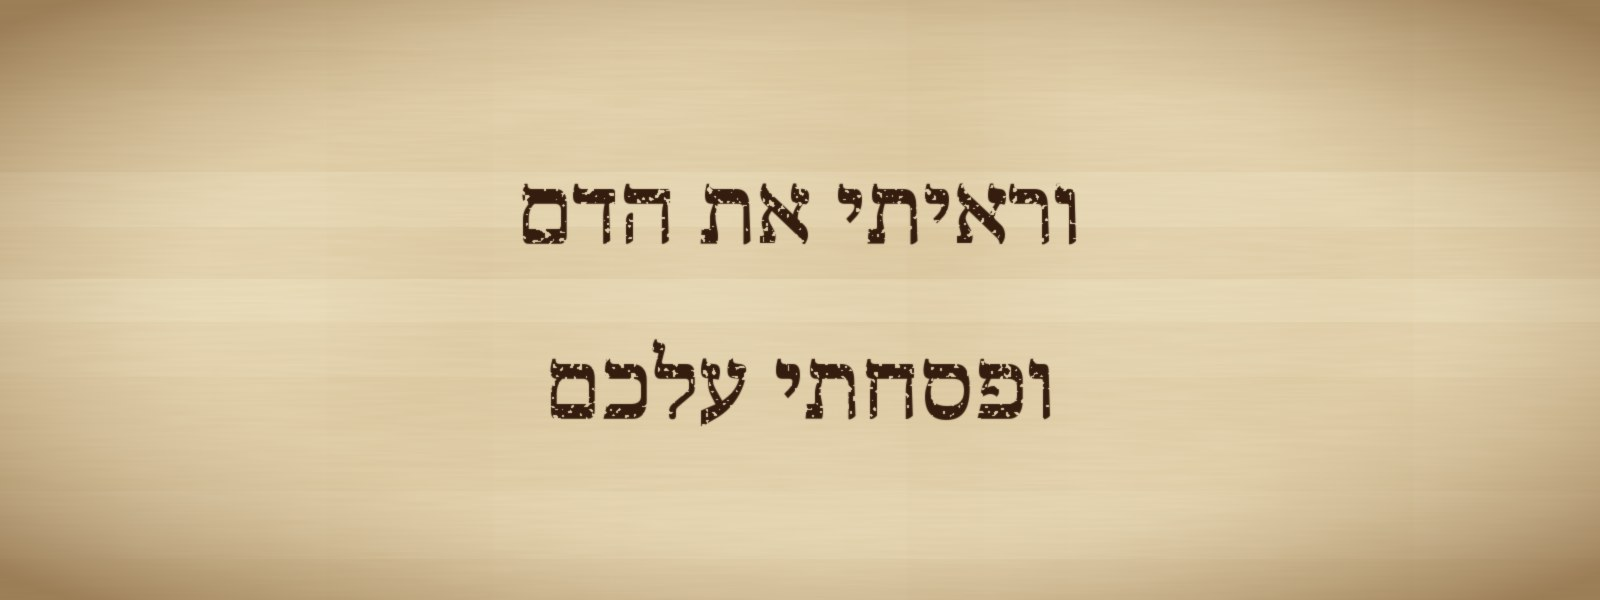
\includegraphics[width=0.80\linewidth,height=0.36\textheight,keepaspectratio]{portada.jpg}\\[-1pt]
  {\fontsize{5}{6}\selectfont\color{sepia}\textit{Nota.} Elaboración propia: Éx 12:13 en texto hebreo consonántico (BHS).}}
\begin{document}
\frame{\titlepage}

\begin{frame}\frametitle{Contenidos}\small\tableofcontents\end{frame}

% ==================================================================
\section{Introducción}


\begin{frame}{Pésaj en el ciclo de Levítico 23}
\centering
\resizebox{0.92\linewidth}{!}{%
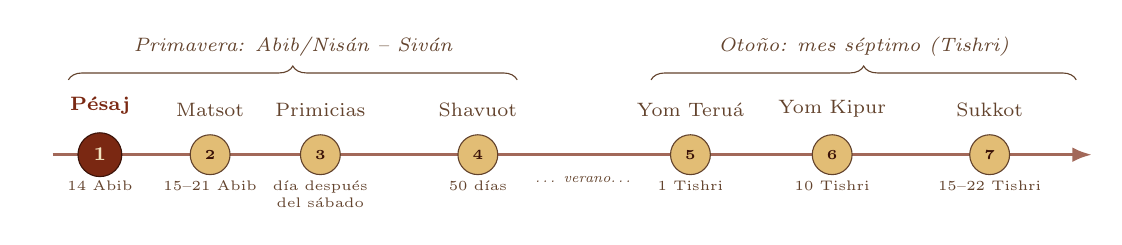
\begin{tikzpicture}[x=1cm,y=1cm,font=\scriptsize]
 \def\fiestaactual{1}
 \draw[line width=1.2pt,tierraroja!70,-{Latex[length=2.5mm]}] (0,0) -- (13.2,0);
 \draw[decorate,decoration={brace,amplitude=5pt},sepia] (0.2,0.95) -- (5.9,0.95) node[midway,above=5pt,font=\scriptsize\itshape]{Primavera: Abib/Nisán -- Siván};
 \draw[decorate,decoration={brace,amplitude=5pt},sepia] (7.6,0.95) -- (13.0,0.95) node[midway,above=5pt,font=\scriptsize\itshape]{Otoño: mes séptimo (Tishri)};
 \foreach \n/\x/\t/\d in {1/0.6/Pésaj/{14 Abib},2/2.0/Matsot/{15--21 Abib},3/3.4/Primicias/{día después del sábado},4/5.4/Shavuot/{50 días},5/8.1/Yom Teruá/{1 Tishri},6/9.9/Yom Kipur/{10 Tishri},7/11.9/Sukkot/{15--22 Tishri}}{
   \ifnum\n=\fiestaactual
     \node[circle,fill=tierraroja,draw=caferojizo,minimum size=5.5mm,text=papiro,font=\scriptsize\bfseries] at (\x,0) {\n};
     \node[above=3pt,font=\scriptsize\bfseries,text=tierraroja] at (\x,0.28) {\t};
   \else
     \node[circle,fill=mostaza!70,draw=sepia,minimum size=4.5mm,text=caferojizo,font=\tiny\bfseries] at (\x,0) {\n};
     \node[above=3pt,text=sepia] at (\x,0.25) {\t};
   \fi
   \node[below=6pt,text width=1.6cm,align=center,font=\tiny,text=sepia] at (\x,0) {\d};}
 \node[font=\tiny\itshape,text=sepia] at (6.75,-0.32) {\ldots\ verano\ldots};
\end{tikzpicture}}\par\medskip
\begin{columns}[t,onlytextwidth]
\begin{column}{0.50\textwidth}
\begin{cita}Este mes os será principio de los meses; para vosotros será éste el primero en los meses del año.\fuente{(Éx 12:2)}\end{cita}
\scriptsize\RaggedRight El año empieza con \destacar{una casa con sangre en la puerta}. Pascua (14) y Ázimos (15--21) son dos solemnidades contiguas (Lc 22:1).
\end{column}
\begin{column}{0.48\textwidth}
\begin{tcolorbox}[colback=papiro,colframe=tierraroja,boxrule=1pt,arc=3pt,fontupper=\scriptsize]
\textbf{Tesis.} La Pascua es el \destacar{memorial de una salvación por sustitución dentro de una casa}: Dios ve la sangre y ``pasa por encima''. El NT reconoce en Jesús al Cordero cuya sangre libra de la muerte (1~Co 5:7).
\end{tcolorbox}
\end{column}
\end{columns}
\end{frame}

% ==================================================================
\section{El texto}

\begin{frame}{Texto ancla: Éx 12:13}
\fotolado{panel_exodo12_13.jpg}{Elaboración propia: Éx 12:13 en texto hebreo consonántico (BHS).}
\begin{columns}[c,onlytextwidth]
\begin{column}{0.57\textwidth}
\begin{cita}Y la sangre os será por señal en las casas donde vosotros estéis; y veré la sangre y pasaré de vosotros, y no habrá en vosotros plaga de mortandad cuando hiera la tierra de Egipto.\fuente{(Éx 12:13)}\end{cita}
\small\RaggedRight Tres tiempos:
\begin{itemize}\small
\item la sangre, \heb{אוֹת} (\emph{ot}), ``señal'' \heb{לָכֶם}, ``para vosotros'';
\item Dios \destacar{ve} y \destacar{pasa}: \heb{וּפָסַחְתִּי} (\emph{ufasajtí});
\item no hay ``plaga para destrucción'' (\heb{לְמַשְׁחִית}).
\end{itemize}
\end{column}
\begin{column}{0.41\textwidth}\end{column}
\end{columns}
\end{frame}

\begin{frame}{Lv 23:5: una sola línea}
\fotolado{panel_levitico23_5.jpg}{Elaboración propia: Lv 23:5 en texto hebreo consonántico (BHS).}
\begin{columns}[c,onlytextwidth]
\begin{column}{0.57\textwidth}
\centering\heb{בֵּין הָעַרְבָּיִם פֶּסַח לַיהוָה}
\begin{cita}En el mes primero, a los catorce del mes, entre las dos tardes, pascua es de \SENOR.\fuente{(Lv 23:5)}\end{cita}
\small\RaggedRight El ``Reglamento del Culto'' solo da \destacar{la fecha y la pertenencia}: \emph{pésaj la-YHWH}, ``pascua para el \SENOR''. Todo lo demás está en Éxodo 12, que el lector ya conoce.
\end{column}
\begin{column}{0.41\textwidth}\end{column}
\end{columns}
\end{frame}

\begin{frame}{El procedimiento de Éxodo 12}
\begin{columns}[t,onlytextwidth]
\begin{column}{0.55\textwidth}
\begin{cita}En el diez de este mes tómese cada uno un cordero\ldots{} El animal será sin defecto, macho de un año\ldots{} Y lo guardaréis hasta el día catorce\ldots{} y lo inmolará toda la congregación\ldots{} entre las dos tardes.\fuente{(Éx 12:3, 5--6)}\end{cita}
\begin{cita}Y lo comeréis así: ceñidos vuestros lomos, vuestro calzado en vuestros pies, y vuestro bordón en vuestra mano; y lo comeréis apresuradamente; es la Pascua de \SENOR.\fuente{(Éx 12:11)}\end{cita}
\end{column}
\begin{column}{0.43\textwidth}\small
\begin{itemize}
\item sangre en los \destacar{dos postes y el dintel} (12:7);
\item carne \destacar{asada al fuego}, \emph{matsot} y hierbas amargas (12:8);
\item nadie sale de casa \destacar{hasta la mañana} (12:22);
\item ``este día os será en \destacar{memoria}\ldots{} por estatuto perpetuo'' (12:14).
\end{itemize}
\end{column}
\end{columns}
\end{frame}

\begin{frame}{Las leyes de la Pascua (1)}
\scriptsize\renewcommand{\arraystretch}{1.15}
\begin{tabular}{@{}L{1.9cm}L{2.6cm}L{7.6cm}@{}}
\toprule
\textbf{Texto} & \textbf{Contexto} & \textbf{Qué añade} \\ \midrule
Éx 12:1--14 & Egipto, antes de la plaga & Nuevo comienzo del año; cordero el 10, inmolado el 14; sangre en la puerta; asado, \emph{matsot}, hierbas amargas; ``memoria''. \\
Éx 12:21--28 & Moisés a los ancianos & Hisopo y lebrillo; el \emph{mashjit} no entra; ``¿Qué es este rito vuestro?''. \\
Éx 12:43--51 & Después de la salida & Ningún incircunciso come; el extranjero circuncidado sí; ``ni quebraréis hueso suyo''. \\
Éx 13:1--16 & Camino a Canaán & Consagración y rescate de los primogénitos; ``lo contarás\ldots{} a tu hijo''. \\
Éx 23:15--18; 34:25 & Pacto y su renovación & Mes de Abib; nada leudado con la sangre; nada queda hasta la mañana. \\
\bottomrule
\end{tabular}\par\medskip
\small\RaggedRight Primer movimiento: de una noche única a una \destacar{memoria perpetua} (Éx 12:14, 17, 24).
\end{frame}

\begin{frame}{Las leyes de la Pascua (2)}
\scriptsize\renewcommand{\arraystretch}{1.15}
\begin{tabular}{@{}L{1.9cm}L{2.6cm}L{7.6cm}@{}}
\toprule
\textbf{Texto} & \textbf{Contexto} & \textbf{Qué añade} \\ \midrule
Lv 23:5 & Reglamento de las solemnidades & Fecha y pertenencia: 14 del mes primero, ``entre las dos tardes''. \\
Nm 9:1--14 & Sinaí, año 2 & Segunda Pascua para el impuro y el viajero; castigo al que no la hace; el extranjero puede celebrarla. \\
Nm 28:16 & Calendario de ofrendas & Fecha; las ofrendas del templo son para los siete días de Ázimos (28:17--25). \\
Dt 16:1--8 & Discurso en Moab & ``En el lugar que \SENOR{} escogiere''; ``ovejas y vacas''; ``a la puesta del sol''; verbo \emph{bashal}. \\
\bottomrule
\end{tabular}\par\medskip
\small\RaggedRight De la \destacar{casa} al \destacar{santuario} (Dt 16:2, 6); de Israel a \destacar{quien se une a Israel} (Éx 12:48; Nm 9:14). Nm 9 crea la \emph{segunda Pascua} (14 del mes segundo): la fecha importa, y la exclusión del impuro no es definitiva.
\end{frame}


\begin{frame}{Dt 16:7: ¿asar o hervir?}
\centering\heb{וּבִשַּׁלְתָּ וְאָכַלְתָּ בַּמָּקוֹם אֲשֶׁר יִבְחַר יְהוָה אֱלֹהֶיךָ בּוֹ}\par\smallskip
\scriptsize\renewcommand{\arraystretch}{1.18}
\begin{tabular}{@{}L{2.0cm}L{4.6cm}L{5.5cm}@{}}
\toprule
\textbf{Texto} & \textbf{Hebreo} & \textbf{Sentido} \\ \midrule
Éx 12:9 & \heb{וּבָשֵׁל מְבֻשָּׁל בַּמָּיִם} & ``ni cocida en agua, sino asada al fuego'' \\
Dt 16:7 & \heb{וּבִשַּׁלְתָּ} \emph{uvishaltá} & \emph{bashal}, ``cocer''; la RVR1960 traduce ``la asarás'' \\
2~Cr 35:13 & \heb{וַיְבַשְּׁלוּ הַפֶּסַח בָּאֵשׁ} & ``asaron la pascua al fuego conforme a la ordenanza'' \\
\bottomrule
\end{tabular}\par\medskip
\small\RaggedRight El cronista usa el verbo de Deuteronomio (\emph{bashal}) con el complemento de Éxodo (``al fuego''): \destacar{la Biblia armoniza la Biblia}.\par\smallskip
\precision{\emph{bashal} puede significar ``cocinar al fuego'' en general (Tigay, 1996); Dt 16:2 (``ovejas y vacas'') se refiere, según la lectura rabínica, a las ofrendas de la semana festiva.}
\end{frame}

% ==================================================================
\section{Historia}

\begin{frame}{Abib y la fecha del éxodo}
\begin{columns}[t,onlytextwidth]
\begin{column}{0.48\textwidth}\small\RaggedRight
\textbf{\textcolor{tierraroja}{El mes de las espigas.}} \heb{אָבִיב} (\emph{aviv}) es la cebada ``espigada'' y verde: ``la cebada estaba ya espigada'' (Éx 9:31). Mes lunar: el 14 es \destacar{luna llena}. Después del exilio se llamó \emph{Nisán} (Neh 2:1; Est 3:7).\par\smallskip
\precision{el calendario judío calculado y la regla del mes intercalar son rabínicos (siglos \textsc{iv}--\textsc{x}).}
\end{column}
\begin{column}{0.50\textwidth}
\centering
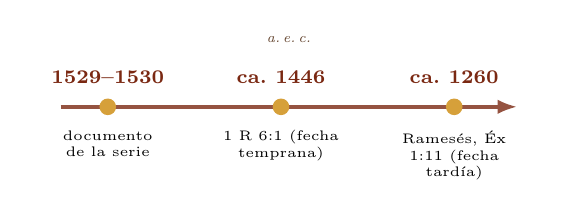
\begin{tikzpicture}[font=\scriptsize]
 \draw[line width=1.3pt,tierraroja!80,-{Latex[length=2.5mm]}] (0,0) -- (5.8,0);
 \foreach \x/\a/\b in {0.6/{1529--1530}/{documento de la serie}, 2.8/{ca.\ 1446}/{1~R 6:1 (fecha temprana)}, 5.0/{ca.\ 1260}/{Ramesés, Éx 1:11 (fecha tardía)}}{
   \fill[mostaza] (\x,0) circle (3pt);
   \node[above=5pt,font=\scriptsize\bfseries,text=tierraroja] at (\x,0) {\a};
   \node[below=5pt,text width=1.8cm,align=center,font=\tiny] at (\x,0) {\b};}
 \node[font=\tiny\itshape,text=sepia] at (2.9,0.85) {a.\,e.\,c.};
\end{tikzpicture}\par\smallskip
\precision{el texto no da una fecha absoluta; ninguna de las tres altera el sentido de la Pascua (Hoffmeier, 1997).}
\end{column}
\end{columns}
\end{frame}

\begin{frame}{Juicio y primogénitos}
\begin{columns}[t,onlytextwidth]
\begin{column}{0.52\textwidth}
\begin{cita}Israel es mi hijo, mi primogénito. Ya te he dicho que dejes ir a mi hijo, para que me sirva\ldots{} he aquí yo voy a matar a tu hijo, tu primogénito.\fuente{(Éx 4:22--23)}\end{cita}
\small\RaggedRight ``Ejecutaré mis juicios en \destacar{todos los dioses de Egipto}'' (Éx 12:12; Nm 33:4). El primogénito del faraón ``que se sentaba sobre su trono'' (12:29) era el heredero del orden divino egipcio.
\end{column}
\begin{column}{0.46\textwidth}\small
\begin{itemize}
\item Esa noche el juicio no distingue por etnia, sino por \destacar{la sangre}.
\item Los librados son de Dios: ``Conságrame todo primogénito'' (Éx 13:2); se rescatan (13:13--15); los levitas los sustituyen (Nm 3:13).
\end{itemize}
\precision{asignar cada plaga a un dios egipcio es a menudo forzado; el texto afirma el juicio ``contra todos los dioses'' (Sarna, 1991).}
\end{column}
\end{columns}
\end{frame}

\begin{frame}{Del 10 al 15 de Abib}
\centering
\resizebox{\linewidth}{!}{%
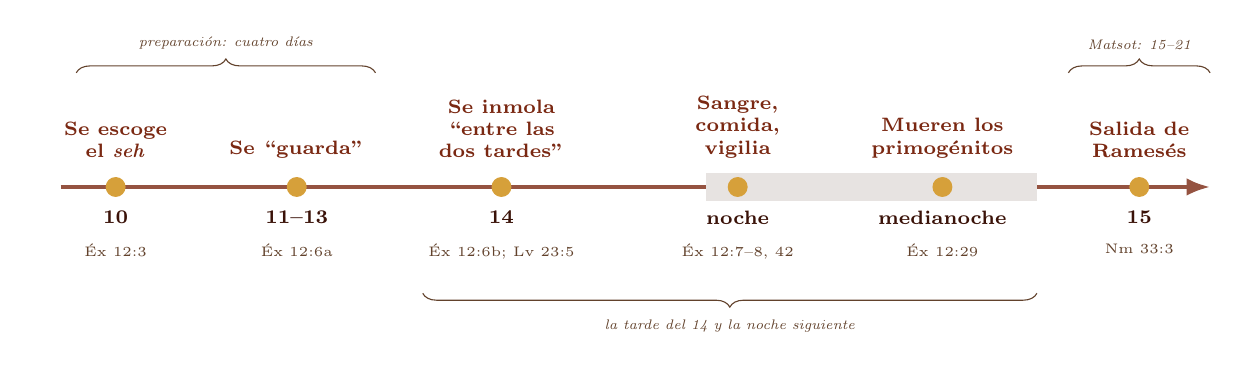
\begin{tikzpicture}[x=1cm,y=1cm,font=\scriptsize]
 \draw[line width=1.4pt,tierraroja!80,-{Latex[length=3mm]}] (0,0) -- (14.6,0);
 \fill[caferojizo!12] (8.2,-0.18) rectangle (12.4,0.18);
 \foreach \x/\d/\t/\r in {0.7/10/{Se escoge el \emph{seh}}/{Éx 12:3}, 3.0/{11--13}/{Se ``guarda''}/{Éx 12:6a}, 5.6/14/{Se inmola ``entre las dos tardes''}/{Éx 12:6b; Lv 23:5}, 8.6/{noche}/{Sangre, comida, vigilia}/{Éx 12:7--8, 42}, 11.2/{medianoche}/{Mueren los primogénitos}/{Éx 12:29}, 13.7/15/{Salida de Ramesés}/{Nm 33:3}}{
   \fill[mostaza] (\x,0) circle (3.6pt);
   \node[above=7pt,text width=2.0cm,align=center,font=\scriptsize\bfseries,text=tierraroja] at (\x,0) {\t};
   \node[below=5pt,font=\scriptsize\bfseries,text=caferojizo] at (\x,0) {\d};
   \node[below=17pt,text width=2.0cm,align=center,font=\tiny,text=sepia] at (\x,0) {\r};}
 \draw[decorate,decoration={brace,amplitude=5pt,mirror},sepia] (4.6,-1.35) -- (12.4,-1.35) node[midway,below=6pt,font=\tiny\itshape,text=sepia]{la tarde del 14 y la noche siguiente};
 \draw[decorate,decoration={brace,amplitude=5pt},sepia] (0.2,1.45) -- (4.0,1.45) node[midway,above=5pt,font=\tiny\itshape,text=sepia]{preparación: cuatro días};
 \draw[decorate,decoration={brace,amplitude=5pt},sepia] (12.8,1.45) -- (14.6,1.45) node[midway,above=5pt,font=\tiny\itshape,text=sepia]{Matsot: 15--21};
\end{tikzpicture}}\par\medskip
\small\RaggedRight \heb{לֵיל שִׁמֻּרִים הוּא לַיהוָה}: ``es \destacar{noche de guardar} para \SENOR'' (Éx 12:42). La palabra \emph{shimurim} aparece dos veces en ese versículo y en ningún otro (conteo propio sobre el Códice de Leningrado): Dios veló sobre Israel, e Israel vela para Dios.
\end{frame}

\begin{frame}{De Ramesés a Sucot}
\begin{columns}[c,onlytextwidth]
\begin{column}{0.56\textwidth}
\centering
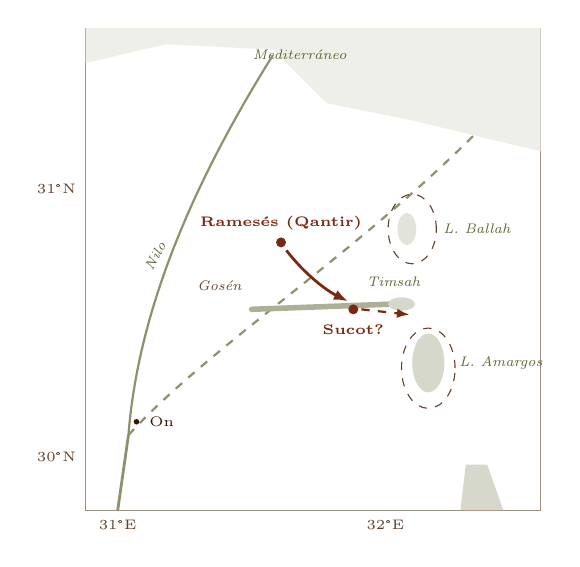
\begin{tikzpicture}[x=3.4cm,y=3.4cm,font=\tiny]
 \draw[sepia!60,line width=0.4pt] (0.1,0) rectangle (1.8,1.8);
 \fill[oliva!10] (0.1,1.67) -- (0.4,1.74) -- (0.8,1.72) -- (1.0,1.52) -- (1.3,1.46) -- (1.8,1.34) -- (1.8,1.8) -- (0.1,1.8) -- cycle;
 \node[font=\tiny\itshape,text=oliva] at (0.9,1.70) {Mediterráneo};
 \draw[oliva!70,line width=1pt] (0.22,0.0) -- (0.26,0.28);
 \draw[oliva!70,line width=0.8pt] (0.26,0.28) .. controls (0.30,0.8) and (0.55,1.3) .. (0.80,1.70);
 \draw[oliva!70,line width=0.8pt,dashed] (0.26,0.28) .. controls (0.55,0.6) and (1.1,0.95) .. (1.55,1.40);
 \node[font=\tiny\itshape,text=oliva,rotate=62] at (0.36,0.95) {Nilo};
 \draw[oliva!50,line width=2pt,line cap=round] (0.72,0.75) -- (1.26,0.77);
 \fill[oliva!25] (1.28,0.77) ellipse (0.05 and 0.025);
 \fill[oliva!25] (1.38,0.55) ellipse (0.06 and 0.11);
 \fill[oliva!25] (1.52,0.17) -- (1.60,0.17) -- (1.66,0.0) -- (1.50,0.0) -- cycle;
 \fill[oliva!18] (1.30,1.05) ellipse (0.035 and 0.06);
 \node[font=\tiny\itshape,text=oliva,anchor=west] at (1.46,0.55) {L.\ Amargos};
 \node[font=\tiny\itshape,text=oliva,anchor=west] at (1.40,1.05) {L.\ Ballah};
 \node[font=\tiny\itshape,text=oliva,anchor=south] at (1.25,0.80) {Timsah};
 \node[font=\tiny\itshape,text=sepia] at (0.60,0.84) {Gosén};
 \fill[caferojizo] (0.29,0.33) circle (1pt) node[anchor=west,text=caferojizo] {\,On};
 \fill[tierraroja] (0.83,1.00) circle (1.8pt) node[anchor=south,font=\tiny\bfseries,text=tierraroja,yshift=1pt] {Ramesés (Qantir)};
 \fill[tierraroja] (1.10,0.75) circle (1.8pt);
 \node[anchor=north,font=\tiny\bfseries,text=tierraroja,yshift=-2pt] at (1.10,0.75) {Sucot?};
 \draw[tierraroja,line width=1pt,-{Latex[length=1.8mm]}] (0.85,0.97) .. controls (0.92,0.88) and (1.0,0.82) .. (1.08,0.78);
 \draw[tierraroja,line width=0.8pt,dashed,-{Latex[length=1.6mm]}] (1.13,0.75) -- (1.31,0.73);
 \draw[sepia,dashed] (1.38,0.53) ellipse (0.10 and 0.15);
 \draw[sepia,dashed] (1.32,1.05) ellipse (0.09 and 0.13);
 \node[below,text=sepia] at (0.22,0) {31°E}; \node[below,text=sepia] at (1.22,0) {32°E};
 \node[left,text=sepia] at (0.1,0.2) {30°N}; \node[left,text=sepia] at (0.1,1.2) {31°N};
\end{tikzpicture}\par
{\fontsize{5}{6}\selectfont\color{sepia}\textit{Nota.} Elaboración propia; coordenadas aproximadas reales. Punteado: ubicaciones discutidas.}
\end{column}
\begin{column}{0.42\textwidth}\small\RaggedRight
``Partieron los hijos de Israel de Ramesés a Sucot'' (Éx 12:37).
\begin{itemize}\small
\item \destacar{Ramesés}: Pi-Ramsés (Qantir, 30,8°N 31,8°E).
\item \destacar{Sucot}: región de Tjeku; Tell el-Maskhuta (30,55°N 32,1°E).
\item Etam, Pi-hahirot, Migdol, Baal-zefón: \destacar{discutidos} (Nm 33:5--7).
\end{itemize}
\precision{la salida fue el día 15 (Nm 33:3); las fechas 16--18 son cálculos de la serie.}
\end{column}
\end{columns}
\end{frame}

\begin{frame}{Las pascuas de la historia}
\scriptsize\renewcommand{\arraystretch}{1.15}
\begin{tabular}{@{}L{2.4cm}L{2.2cm}L{7.5cm}@{}}
\toprule
\textbf{Texto} & \textbf{Ocasión} & \textbf{Rasgos} \\ \midrule
Jos 5:10--12 & Gilgal & Tras la circuncisión; al otro día, fruto de la tierra; \destacar{cesa el maná}. \\
2~Cr 30 & Ezequías & En el \destacar{mes segundo} (Nm 9); intercede por los impuros y ``sanó al pueblo'' (30:20). \\
2~R 23:21--23; 2~Cr 35 & Josías & ``Conforme\ldots{} al libro de este pacto''; levitas degüellan, sacerdotes rocían la sangre. \\
Esd 6:19--22 & Regreso, 515 a.\,e.\,c. & Tras dedicar el segundo templo; comen los purificados. \\
Ez 45:21--24 & Templo futuro & ``Fiesta de siete días''; el príncipe ofrece un becerro \destacar{por el pecado}. \\
\bottomrule
\end{tabular}\par\medskip
\small\RaggedRight Cada nueva etapa de Israel empieza con una Pascua: ``no había sido hecha tal pascua desde los tiempos en que los jueces gobernaban a Israel'' (2~R 23:22).
\end{frame}

\begin{frame}{En el Segundo Templo}
\begin{columns}[t,onlytextwidth]
\begin{column}{0.55\textwidth}\small
\begin{itemize}
\item \textbf{Josefo}: \grc{πάσχα} significa \grc{ὑπερβάσια}, ``paso por encima'' (\emph{Ant.} 2.313); unas 255\,600 víctimas entre la hora 9 y la 11, diez comensales por víctima (\emph{Guerra} 6.423--427).
\item \textbf{Filón}: \grc{διαβατήρια}, ``fiesta del cruce''; todo el pueblo actúa como sacerdote (\emph{Spec.} 2.145).
\item \textbf{Misná}: tres turnos, \emph{Hallel} durante la matanza (m.~Pesajim 5).
\end{itemize}
\end{column}
\begin{column}{0.43\textwidth}
\precision{la cifra de Josefo es suya y probablemente inflada. La Misná es posterior al 70 e.\,c. El \emph{séder} con cuatro copas y \emph{Hagadá} es un desarrollo rabínico posterior al templo (Bokser, 1984); la última cena es anterior a esa forma.}\par\medskip
\precision{el papiro pascual de Elefantina (419 a.\,e.\,c.) regula los Ázimos del 15 al 21 de Nisán; la palabra ``pascua'' está restituida (Porten \& Yardeni, 1986).}
\end{column}
\end{columns}
\end{frame}

% ==================================================================
\section{Filología}

\begin{frame}{\heb{פֶּסַח} (\emph{pésaj}): tres sentidos}
\centering
\resizebox{0.96\linewidth}{!}{%
\begin{tikzpicture}[font=\scriptsize]
 \node[draw=tierraroja,line width=1pt,fill=papiro,rounded corners=4pt,inner sep=6pt,align=center] (c) at (0,0) {\Large\heb{פ־ס־ח}\\[2pt]\small\emph{p-s-j}};
 \node[caja,text width=3.4cm,align=left] (a) at (-4.1,1.15) {\textbf{\textcolor{tierraroja}{pasar por encima, saltar}}\\ ``pasaré de vosotros'' (Éx 12:13, 23, 27); ``saltaban'' (1~R 18:26)};
 \node[caja,text width=3.4cm,align=left] (b) at (4.1,1.15) {\textbf{\textcolor{tierraroja}{cojear, vacilar}}\\ ``¿hasta cuándo claudicaréis\ldots?'' (1~R 18:21); \emph{piséaj}, ``cojo'' (2~S 9:13)};
 \node[caja,text width=3.4cm,align=left] (d) at (0,-1.55) {\textbf{\textcolor{tierraroja}{proteger, amparar}}\\ \heb{פָּסֹחַ} ``preservando'' (Is 31:5), como aves sobre el nido};
 \draw[-{Latex[length=2mm]},mostaza!85!tierraroja,line width=1.1pt] (c) -- (a);
 \draw[-{Latex[length=2mm]},mostaza!85!tierraroja,line width=1.1pt] (c) -- (b);
 \draw[-{Latex[length=2mm]},mostaza!85!tierraroja,line width=1.1pt] (c) -- (d);
\end{tikzpicture}}\par\medskip
\scriptsize\RaggedRight LXX: \grc{σκεπάσω}, ``protegeré'' (12:13), y \grc{παρελεύσεται}, ``pasará de largo'' (12:23). Onqelos: ``tendré piedad''. Rashi: ``tendré compasión'', pero ``todo \emph{pesijá} es lenguaje de salto''. Los sentidos se suman: Dios \destacar{salta} la puerta y \destacar{guarda} la casa.
\end{frame}

\begin{frame}{``Entre las dos tardes''}
\centering\heb{בֵּין הָעַרְבָּיִם}\quad \emph{bein ha'arbayim} (Éx 12:6; Lv 23:5; Nm 9:3)\par\medskip
\scriptsize\renewcommand{\arraystretch}{1.2}
\begin{tabular}{@{}L{3.5cm}L{5.2cm}L{3.3cm}@{}}
\toprule
\textbf{Lectura} & \textbf{Fundamento} & \textbf{Quiénes} \\ \midrule
Del declinar del sol hasta la puesta & Josefo: hora 9--11; Misná: después del \emph{tamid} (m.~Pesajim 5:1) & Fariseos, rabinos; Rashi \\
Entre la puesta y la oscuridad & Dt 16:6: ``a la puesta del sol'' & Samaritanos, caraítas; Ibn Ezra \\
Al anochecer que \emph{abre} el 14 & La cena de Jesús la noche antes de morir & Iglesias de Dios; la serie \\
\bottomrule
\end{tabular}\par\medskip
\small\RaggedRight La misma expresión fija el sacrificio vespertino diario (Éx 29:39) y el encendido de las lámparas (Éx 30:8).
\end{frame}

\begin{frame}{Palabras de la noche}
\scriptsize\renewcommand{\arraystretch}{1.16}
\begin{tabular}{@{}L{2.9cm}L{9.2cm}@{}}
\toprule
\textbf{Palabra} & \textbf{Sentido y uso} \\ \midrule
\heb{שֶׂה תָמִים} \emph{seh tamim} & res menor \destacar{íntegra}, ``de las ovejas o de las cabras'' (Éx 12:5); \emph{tamim} = apto para el altar; cf.\ \grc{ἀμνοῦ ἀμώμου} (1~P 1:19). \\
\heb{דָּם} \emph{dam} / \heb{אוֹת} \emph{ot} & la sangre como \destacar{señal} ``para vosotros'' (12:13): como el arco iris, la circuncisión y el sábado; Dios ``ve'' la sangre. \\
\heb{הַמַּשְׁחִית} \emph{hamashjit} & ``el destructor'' (12:23); 2~S 24:16; \grc{ὁ ὀλοθρεύων} (He 11:28), \grc{ὁ ὀλοθρευτής} (1~Co 10:10). \\
\heb{מְרֹרִים} \emph{merorim} & ``hierbas amargas'' (12:8), raíz de ``\destacar{amargaron} su vida'' (\heb{וַיְמָרְרוּ}, Éx 1:14). \\
\heb{זִכָּרוֹן} \emph{zikarón} & ``memoria'' hecha acto (12:14); LXX \grc{μνημόσυνον}; ``en memoria de mí'', \grc{ἀνάμνησιν} (Lc 22:19). \\
\heb{חֻקַּת עוֹלָם} \emph{jukat olam} & ``estatuto perpetuo'' (12:14, 17); la fórmula de cada fiesta en Lv 23. \\
\bottomrule
\end{tabular}\par\smallskip
\precision{``sangre'' aparece seis veces en Éx 12:7--23 (vv. 7, 13 [2×], 22 [2×], 23): conteo propio sobre el Códice de Leningrado.}
\end{frame}

\begin{frame}{La puerta de Éxodo 12}
\centering
\resizebox{!}{0.68\textheight}{%
\begin{tikzpicture}[x=1cm,y=1cm,font=\scriptsize]
 \fill[sepia!10] (-3.2,0) rectangle (3.2,4.6);
 \draw[sepia!50] (-3.2,0) rectangle (3.2,4.6);
 \fill[caferojizo!75] (-1.0,0) rectangle (1.0,3.3);
 \fill[mostaza!55,draw=sepia] (-1.35,0) rectangle (-1.0,3.3);
 \fill[mostaza!55,draw=sepia] (1.0,0) rectangle (1.35,3.3);
 \fill[mostaza!65,draw=sepia] (-1.6,3.3) rectangle (1.6,3.72);
 \foreach \y in {1.4,1.9,2.4} {\draw[tierraroja,line width=2.2pt,line cap=round] (-1.18,\y) -- (-1.18,\y+0.28); \draw[tierraroja,line width=2.2pt,line cap=round] (1.18,\y) -- (1.18,\y+0.28);}
 \foreach \x in {-0.9,-0.3,0.3,0.9} {\draw[tierraroja,line width=2.2pt,line cap=round] (\x,3.51) -- (\x+0.3,3.51);}
 \fill[sepia!45,draw=sepia] (-1.6,-0.14) rectangle (1.6,0.0);
 \draw[sepia,fill=sepia!20] (1.9,0.0) .. controls (1.95,-0.35) and (2.55,-0.35) .. (2.6,0.0) -- cycle;
 \fill[tierraroja!80] (1.98,-0.04) .. controls (2.05,-0.2) and (2.45,-0.2) .. (2.52,-0.04) -- cycle;
 \draw[oliva,line width=0.8pt] (2.25,0.05) -- (2.0,1.1);
 \foreach \a in {100,120,140,80} {\draw[oliva,line width=0.5pt] (2.0,1.1) -- ++(\a:0.3);}
 \draw[sepia,-{Latex[length=1.6mm]}] (-4.4,3.9) node[anchor=east,align=right,text=caferojizo] {dintel\\ \heb{מַשְׁקוֹף}} -- (-1.5,3.55);
 \draw[sepia,-{Latex[length=1.6mm]}] (-4.4,1.9) node[anchor=east,align=right,text=caferojizo] {dos postes\\ \heb{שְׁתֵּי הַמְּזוּזֹת}} -- (-1.3,1.9);
 \draw[sepia,-{Latex[length=1.6mm]}] (-4.4,0.1) node[anchor=east,align=right,text=caferojizo] {umbral / lebrillo\\ \heb{סַף} (12:22)} -- (-1.5,-0.07);
 \draw[sepia,-{Latex[length=1.6mm]}] (4.6,1.0) node[anchor=west,align=left,text=caferojizo] {hisopo\\ \heb{אֵזוֹב} (cf.\ Jn 19:29)} -- (2.1,0.9);
 \draw[sepia,-{Latex[length=1.6mm]}] (4.6,0.0) node[anchor=west,align=left,text=caferojizo] {sangre: ``señal''\\ \heb{לְאֹת} (12:13)} -- (2.45,-0.12);
 \draw[tierraroja,line width=1pt,dashed,-{Latex[length=2.4mm]}] (-3.6,5.0) .. controls (-1.0,6.0) and (1.0,6.0) .. (3.6,5.0);
 \node[text=tierraroja,font=\scriptsize\bfseries,align=center] at (0,6.05) {\heb{וּפָסַח יְהוָה עַל־הַפֶּתַח} \quad ``pasará el \SENOR{} aquella puerta'' (Éx 12:23)};
 \node[text=papiro,font=\scriptsize\itshape,align=center,text width=1.8cm] at (0,1.5) {dentro: la familia, hasta la mañana};
 \node[text=sepia,font=\tiny\itshape,align=center] at (0,4.25) {``no dejará entrar al \emph{mashjit}''};
\end{tikzpicture}}\par
{\fontsize{5}{6}\selectfont\color{sepia}\textit{Nota.} Elaboración propia; esquema sin escala. LXX en 12:22: \grc{παρὰ τὴν θύραν}, ``junto a la puerta''.}
\end{frame}

\begin{frame}{De \emph{pésaj} a ``pascua''}
\centering
\resizebox{\linewidth}{!}{%
\begin{tikzpicture}[font=\scriptsize,
  eslabon/.style={draw=tierraroja,line width=0.7pt,fill=papiro,rounded corners=3pt,text width=2.55cm,align=center,inner sep=4pt,minimum height=1.55cm},
  flecha/.style={-{Latex[length=2.4mm]},mostaza!85!tierraroja,line width=1.2pt}]
 \node[eslabon] (a) at (0,0) {\heb{פֶּסַח}\\ \emph{pésaj}\\[1pt] {\tiny fiesta, víctima y comida}};
 \node[eslabon] (b) at (3.2,0) {\heb{פַּסְחָא}\\ \emph{pasja} (arameo)\\[1pt] {\tiny forma hablada}};
 \node[eslabon] (c) at (6.4,0) {\grc{πάσχα}\\ LXX\\[1pt] {\tiny transcripción (Éx 12:11)}};
 \node[eslabon] (d) at (9.6,0) {\grc{τὸ πάσχα ἡμῶν ἐτύθη Χριστός}\\[1pt] {\tiny 1~Co 5:7}};
 \node[eslabon] (e) at (12.8,0) {\emph{pascua}\\ español\\[1pt] {\tiny vía latín \emph{pascha}}};
 \draw[flecha] (a) -- (b); \draw[flecha] (b) -- (c); \draw[flecha] (c) -- (d); \draw[flecha] (d) -- (e);
 \node[draw=sepia,dashed,rounded corners=2pt,text width=4.6cm,align=center,font=\tiny,text=sepia,inner sep=3pt] (m) at (6.4,-1.75) {\grc{πάσχω} ``padecer'': etimología popular (Melitón, \emph{Sobre la Pascua} 46); eco en Lc 22:15};
 \draw[sepia,dashed,-{Latex[length=1.8mm]}] (m) -- (c);
\end{tikzpicture}}\par\medskip
\small\RaggedRight Pablo toma la palabra exacta de la Torá griega, con su artículo, y \destacar{la aplica a una persona}. En Crónicas la LXX transcribe \grc{φασεκ} (2~Cr 30:1).\par\smallskip
\precision{\grc{πάσχα} es semítica; el juego con \grc{πάσχω} es retórico. Pero Lucas ya junta \grc{τὸ πάσχα φαγεῖν} y \grc{πρὸ τοῦ με παθεῖν} (Lc 22:15).}
\end{frame}

\begin{frame}{``Nuestra pascua'' (1 Co 5:7)}
\fotolado{panel_1corintios5.jpg}{Elaboración propia: 1~Co 5:7 en escritura uncial (texto NA28).}
\begin{columns}[c,onlytextwidth]
\begin{column}{0.57\textwidth}
\begin{cita}Limpiaos, pues, de la vieja levadura, para que seáis nueva masa, sin levadura como sois; porque nuestra pascua, que es Cristo, ya fue sacrificada por nosotros.\fuente{(1~Co 5:7)}\end{cita}
\scriptsize\RaggedRight
\begin{itemize}\scriptsize
\item \grc{ἀμνός}: cordero sacrificial de la LXX; Jn 1:29, 36; Hch 8:32; 1~P 1:19.
\item \grc{ἀρνίον}: casi solo en Apocalipsis (29 veces, más Jn 21:15; conteo propio, SBLGNT): el Cordero ``como inmolado'' (Ap 5:6).
\end{itemize}
\end{column}
\begin{column}{0.41\textwidth}\end{column}
\end{columns}
\end{frame}

% ==================================================================
\section{Texto}

\begin{frame}{Dos problemas de texto}
\begin{columns}[t,onlytextwidth]
\begin{column}{0.48\textwidth}
\textbf{\small\textcolor{tierraroja}{Éx 12:40: los 430 años}}\par\smallskip
\scriptsize\renewcommand{\arraystretch}{1.12}
\begin{tabular}{@{}L{1.3cm}L{4.1cm}@{}}
\toprule
TM & ``en Egipto'' 430 años \\
LXX & ``en la tierra de Egipto \emph{y en la tierra de Canaán}'' \\
PS & ``en Canaán y en Egipto'' \\
\bottomrule
\end{tabular}\par\smallskip
\RaggedRight Con la LXX y el PS, los 430 años se cuentan desde Abraham (Josefo, \emph{Ant.} 2.318; cf.\ Gá 3:17). La RVR1960 sigue al TM.
\end{column}
\begin{column}{0.50\textwidth}
\textbf{\small\textcolor{tierraroja}{Jn 19:36: ``no será quebrado hueso suyo''}}\par\smallskip
\scriptsize\renewcommand{\arraystretch}{1.12}
\begin{tabular}{@{}L{1.7cm}L{4.1cm}@{}}
\toprule
Éx 12:46 & \grc{ὀστοῦν οὐ συντρίψετε ἀπ᾿ αὐτοῦ} \\
Nm 9:12 & \grc{ὀστοῦν οὐ συντρίψουσιν ἀπ᾿ αὐτοῦ} \\
Sal 34:20 [34:21] & \grc{ἓν ἐξ αὐτῶν οὐ συντριβήσεται} \\
Jn 19:36 & \grc{ὀστοῦν οὐ συντριβήσεται αὐτοῦ} \\
\bottomrule
\end{tabular}\par\smallskip
\RaggedRight Juan une la \destacar{ley pascual} (sustantivo, pronombre) y el \destacar{salmo del justo} (voz pasiva).
\end{column}
\end{columns}
\end{frame}

\begin{frame}{¿El 14 o el 15?}
\begin{columns}[t,onlytextwidth]
\begin{column}{0.49\textwidth}
\begin{tcolorbox}[colback=papiro,colframe=mostaza!85!tierraroja,boxrule=0.8pt,arc=2pt,title={Al comenzar el 14},fonttitle=\bfseries\scriptsize,coltitle=caferojizo,colbacktitle=mostaza!35,fontupper=\scriptsize]
\begin{itemize}\scriptsize
\item Sacrificio ``el día 14'' (Éx 12:6; Lv 23:5), ``a la puesta del sol'' (Dt 16:6).
\item Jesús come con los suyos la noche anterior a su muerte.
\item La \emph{leil shimurim} (12:42) sería la noche del 15.
\item Práctica de la serie y de las Iglesias de Dios.
\end{itemize}
\end{tcolorbox}
\end{column}
\begin{column}{0.49\textwidth}
\begin{tcolorbox}[colback=papiro,colframe=mostaza!85!tierraroja,boxrule=0.8pt,arc=2pt,title={Al terminar el 14 (cena en el 15)},fonttitle=\bfseries\scriptsize,coltitle=caferojizo,colbacktitle=mostaza!35,fontupper=\scriptsize]
\begin{itemize}\scriptsize
\item Salida ``el segundo día de la pascua'', el 15, a la vista de los egipcios (Nm 33:3).
\item ``De noche'' te sacó (Dt 16:1).
\item Ázimos desde el 14 ``por la tarde'' (Éx 12:18).
\item Práctica del templo (Josefo; Misná).
\end{itemize}
\end{tcolorbox}
\end{column}
\end{columns}
\precision{las dos reconstrucciones se apoyan en partes del texto; la Biblia no zanja el punto de modo explícito.}
\end{frame}

\begin{frame}{La fecha de la última cena}
\scriptsize\renewcommand{\arraystretch}{1.12}
\begin{tabular}{@{}L{3.0cm}L{6.0cm}L{3.0cm}@{}}
\toprule
\textbf{Postura} & \textbf{Argumento} & \textbf{Autores} \\ \midrule
Cena pascual (sinópticos) & Noche, vino, himno, interpretación de los elementos (Mr 14:12--26) & Jeremias (1966) \\
Antes de la Pascua (Juan) & ``Antes de la fiesta'' (Jn 13:1); ``para\ldots{} comer la pascua'' (18:28); ``preparación de la pascua'' (19:14) & Meier (1991); Brown (1994) \\
Dos calendarios & Calendario solar de 364 días (Qumrán, Jubileos): cena el martes & Jaubert (1957); VanderKam (1998) \\
Otro cómputo & Cena pascual el miércoles; muerte jueves o viernes & Humphreys (2011) \\
Crucifixión el miércoles & ``Tres días y tres noches'' (Mt 12:40); dos sábados & Iglesias de Dios; Baker (2013) \\
\bottomrule
\end{tabular}\par\medskip
\small\RaggedRight Lo común a todos: Jesús muere \destacar{en el tiempo de la Pascua} y es presentado como su víctima.
\end{frame}

\begin{frame}{La semana de la Pasión}
\centering
\resizebox{\linewidth}{!}{%
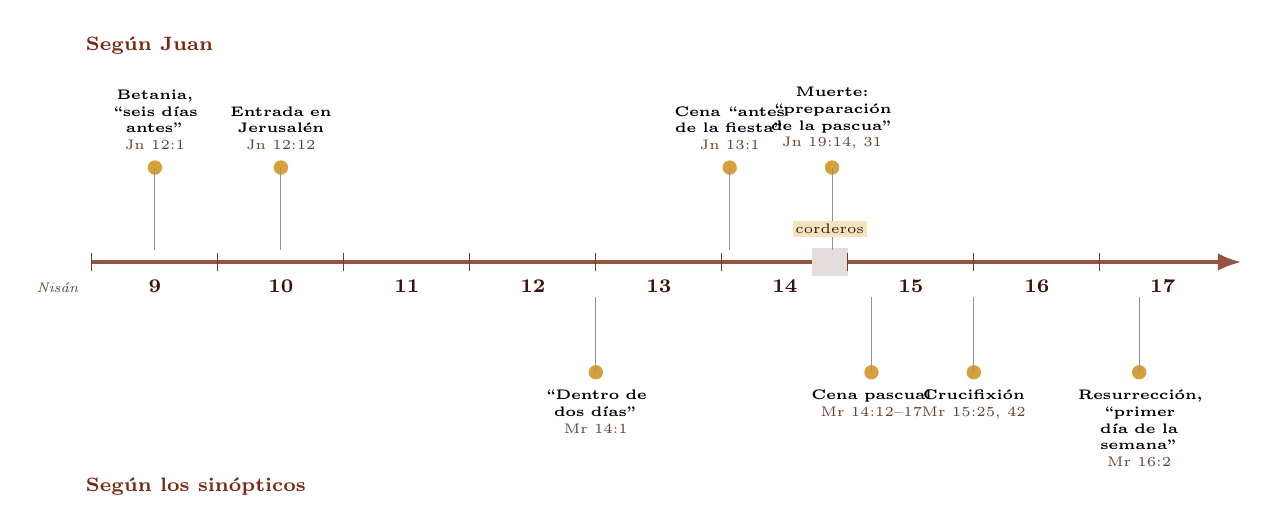
\begin{tikzpicture}[x=1cm,y=1cm,font=\scriptsize]
 \draw[line width=1.4pt,tierraroja!80,-{Latex[length=3mm]}] (0,0) -- (14.6,0);
 \fill[caferojizo!14] (9.15,-0.18) rectangle (9.6,0.18);
 \foreach \x/\d in {0.8/9,2.4/10,4.0/11,5.6/12,7.2/13,8.8/14,10.4/15,12.0/16,13.6/17}{
   \draw[sepia] (\x-0.8,-0.12) -- (\x-0.8,0.12);
   \node[below=3pt,font=\scriptsize\bfseries,text=caferojizo] at (\x,0) {\d};}
 \node[font=\tiny\itshape,text=sepia,anchor=east] at (-0.05,-0.33) {Nisán};
 \node[font=\scriptsize\bfseries,text=tierraroja,anchor=west] at (-0.2,2.75) {Según Juan};
 \foreach \x/\t/\r in {0.8/{Betania, ``seis días antes''}/{Jn 12:1}, 2.4/{Entrada en Jerusalén}/{Jn 12:12}, 8.1/{Cena ``antes de la fiesta''}/{Jn 13:1}, 9.4/{Muerte: ``preparación de la pascua''}/{Jn 19:14, 31}}{
   \fill[mostaza] (\x,1.2) circle (2.6pt);
   \draw[sepia!60] (\x,1.2) -- (\x,0.15);
   \node[above=3pt,text width=1.55cm,align=center,font=\tiny] at (\x,1.2) {\textbf{\t}\\ {\color{sepia}\r}};}
 \node[font=\scriptsize\bfseries,text=tierraroja,anchor=west] at (-0.2,-2.85) {Según los sinópticos};
 \foreach \x/\t/\r in {6.4/{``Dentro de dos días''}/{Mr 14:1}, 9.9/{Cena pascual}/{Mr 14:12--17}, 11.2/{Crucifixión}/{Mr 15:25, 42}, 13.3/{Resurrección, ``primer día de la semana''}/{Mr 16:2}}{
   \fill[mostaza] (\x,-1.4) circle (2.6pt);
   \draw[sepia!60] (\x,-1.4) -- (\x,-0.45);
   \node[below=3pt,text width=1.55cm,align=center,font=\tiny] at (\x,-1.4) {\textbf{\t}\\ {\color{sepia}\r}};}
 \node[font=\tiny,text=caferojizo,fill=papiro,inner sep=1pt] at (9.37,0.42) {corderos};
\end{tikzpicture}}\par\smallskip
{\fontsize{5}{6}\selectfont\color{sepia}\textit{Nota.} Elaboración propia. Días de atardecer a atardecer; asignación aproximada. Franja: la tarde del 14.}
\end{frame}

% ==================================================================
\section{Literatura}

\begin{frame}{La forma de Éxodo 12--13}
\begin{columns}[c,onlytextwidth]
\begin{column}{0.66\textwidth}
\centering
\resizebox{\linewidth}{!}{%
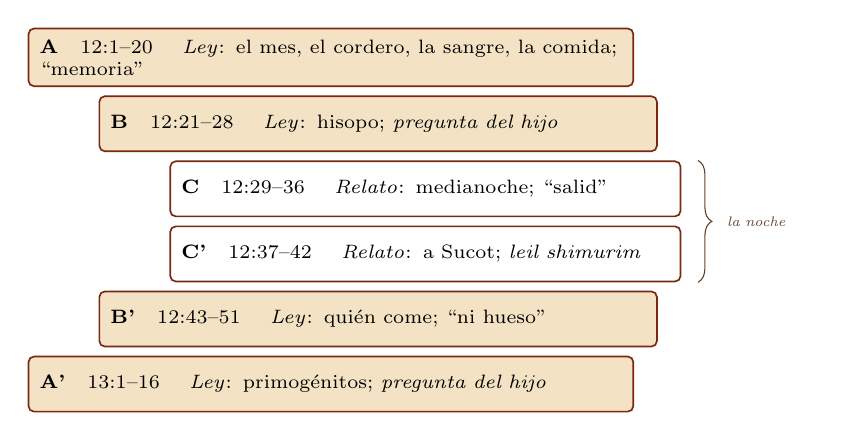
\begin{tikzpicture}[font=\scriptsize,
  bloque/.style={draw=tierraroja,line width=0.6pt,rounded corners=2pt,align=left,inner sep=4pt,minimum height=0.7cm},
  ley/.style={bloque,fill=mostaza!30}, relato/.style={bloque,fill=white}]
 \node[ley,text width=7.4cm] (a) at (0,0) {\textbf{A}\quad 12:1--20 \quad \emph{Ley}: el mes, el cordero, la sangre, la comida; ``memoria''};
 \node[ley,text width=6.8cm,below=3pt of a,xshift=0.6cm] (b) {\textbf{B}\quad 12:21--28 \quad \emph{Ley}: hisopo; \emph{pregunta del hijo}};
 \node[relato,text width=6.2cm,below=3pt of b,xshift=0.6cm] (c) {\textbf{C}\quad 12:29--36 \quad \emph{Relato}: medianoche; ``salid''};
 \node[relato,text width=6.2cm,below=3pt of c] (c2) {\textbf{C'}\quad 12:37--42 \quad \emph{Relato}: a Sucot; \emph{leil shimurim}};
 \node[ley,text width=6.8cm,below=3pt of c2,xshift=-0.6cm] (b2) {\textbf{B'}\quad 12:43--51 \quad \emph{Ley}: quién come; ``ni hueso''};
 \node[ley,text width=7.4cm,below=3pt of b2,xshift=-0.6cm] (a2) {\textbf{A'}\quad 13:1--16 \quad \emph{Ley}: primogénitos; \emph{pregunta del hijo}};
 \draw[decorate,decoration={brace,amplitude=5pt},sepia] ([xshift=6pt]c.north east) -- ([xshift=6pt]c2.south east) node[midway,right=7pt,font=\tiny\itshape,text=sepia,text width=1.3cm]{la noche};
\end{tikzpicture}}\par
{\fontsize{5}{6}\selectfont\color{sepia}\textit{Nota.} Elaboración propia; estructura propuesta. Amarillo: ley; blanco: relato.}
\end{column}
\begin{column}{0.32\textwidth}\small\RaggedRight
El relato \destacar{se detiene} para dictar leyes, y las leyes \destacar{se interrumpen} para contar.\par\smallskip
La historia se vuelve liturgia; la liturgia recuerda la historia.\par\smallskip
\precision{la disposición concéntrica es una propuesta (cf.\ Propp, 1999); lo seguro es la alternancia.}
\end{column}
\end{columns}
\end{frame}

\begin{frame}{``¿Qué rito es este?''}
\fotolado{panel_exodo12_26.jpg}{Elaboración propia: Éx 12:26--27 en texto hebreo consonántico (BHS).}
\begin{columns}[c,onlytextwidth]
\begin{column}{0.57\textwidth}
\begin{cita}Y cuando os dijeren vuestros hijos: ¿Qué es este rito vuestro?, vosotros responderéis: Es la víctima de la pascua de \SENOR, el cual pasó por encima de las casas de los hijos de Israel en Egipto\ldots{} y libró nuestras casas.\fuente{(Éx 12:26--27)}\end{cita}
\scriptsize\RaggedRight ``Rito'' traduce \heb{עֲבֹדָה} (\emph{avodá}), la palabra de la ``dura \destacar{servidumbre}'' (\heb{בַּעֲבֹדָה קָשָׁה}, Éx 1:14). Dios dijo: ``deja ir a mi hijo, \destacar{para que me sirva}'' (4:23). Israel cambia de amo: de los ladrillos al servicio de Dios.
\end{column}
\begin{column}{0.41\textwidth}\end{column}
\end{columns}
\end{frame}

\begin{frame}{Las preguntas de los hijos}
\scriptsize\renewcommand{\arraystretch}{1.14}
\begin{tabular}{@{}L{1.9cm}L{3.4cm}L{6.8cm}@{}}
\toprule
\textbf{Texto} & \textbf{Pregunta} & \textbf{Respuesta} \\ \midrule
Éx 12:26--27 & ``¿Qué es este rito vuestro?'' & ``Es la víctima de la pascua\ldots{} y libró \destacar{nuestras} casas''. \\
Éx 13:8 & (sin pregunta) & ``Se hace esto con motivo de lo que \SENOR{} hizo \destacar{conmigo}''. \\
Éx 13:14 & ``¿Qué es esto?'' & ``\SENOR{} nos sacó con mano fuerte de Egipto''. \\
Dt 6:20--25 & ``¿Qué significan los testimonios\ldots?'' & ``Nosotros éramos siervos de Faraón''. \\
\bottomrule
\end{tabular}\par\medskip
\small\RaggedRight El padre \destacar{cuenta una historia en primera persona}. El credo de Dt 26:5--9 hace lo mismo. Y el profeta invierte la prisa: si se comió ``apresuradamente'' (\heb{בְּחִפָּזוֹן}, Éx 12:11), en el nuevo éxodo ``no saldréis apresurados\ldots{} porque \SENOR{} irá delante de vosotros'' (Is 52:12).
\end{frame}

% ==================================================================
\section{La serie}

\begin{frame}{Reglamento de culto y santuario}
\centering
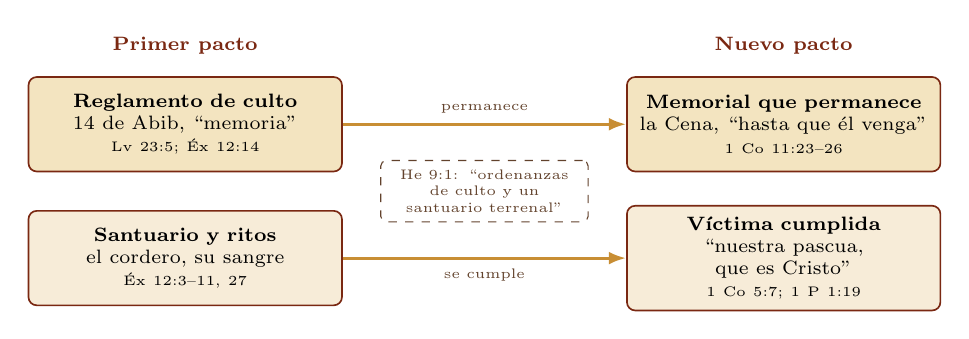
\begin{tikzpicture}[font=\scriptsize,
  col/.style={draw=tierraroja,line width=0.6pt,fill=papiro,rounded corners=3pt,text width=3.7cm,align=center,inner sep=4pt,minimum height=1.2cm},
  fl/.style={-{Latex[length=2.2mm]},mostaza!85!tierraroja,line width=1.1pt}]
 \node[font=\scriptsize\bfseries,text=tierraroja] at (0,1.2) {Primer pacto};
 \node[font=\scriptsize\bfseries,text=tierraroja] at (7.6,1.2) {Nuevo pacto};
 \node[col] (r1) at (0,0.2) {\textbf{Reglamento de culto}\\ 14 de Abib, ``memoria''\\ {\tiny Lv 23:5; Éx 12:14}};
 \node[col,fill=mostaza!20] (s1) at (0,-1.5) {\textbf{Santuario y ritos}\\ el cordero, su sangre\\ {\tiny Éx 12:3--11, 27}};
 \node[col] (r2) at (7.6,0.2) {\textbf{Memorial que permanece}\\ la Cena, ``hasta que él venga''\\ {\tiny 1~Co 11:23--26}};
 \node[col,fill=mostaza!20] (s2) at (7.6,-1.5) {\textbf{Víctima cumplida}\\ ``nuestra pascua, que es Cristo''\\ {\tiny 1~Co 5:7; 1~P 1:19}};
 \draw[fl] (r1) -- node[above,font=\tiny,text=sepia]{permanece} (r2);
 \draw[fl] (s1) -- node[below,font=\tiny,text=sepia]{se cumple} (s2);
 \node[draw=sepia,dashed,rounded corners=2pt,font=\tiny,text=sepia,text width=2.4cm,align=center] at (3.8,-0.65) {He 9:1: ``ordenanzas de culto y un santuario terrenal''};
\end{tikzpicture}\par\medskip
\small\RaggedRight El documento de referencia: el 14 de Abib ``era un día especial\ldots{} de acuerdo al Reglamento de Culto; pero este Reglamento nada decía respecto a que debía sacrificarse un cordero''. Eso está en Éxodo 12.
\end{frame}

\begin{frame}{\emph{Moadim}: citas y reloj}
\begin{columns}[t,onlytextwidth]
\begin{column}{0.52\textwidth}
\centering\small\heb{מוֹעֲדֵי יְהוָה}\ \foreignlanguage{spanish}{[\ldots]}\ \heb{מִקְרָאֵי קֹדֶשׁ}
\begin{cita}Las fiestas solemnes de \SENOR, las cuales proclamaréis como santas convocaciones, serán estas.\fuente{(Lv 23:2)}\end{cita}
\scriptsize\RaggedRight \heb{מִקְרָא} (\emph{mikrá}, Strong H4744): ``convocación, reunión pública'' y también ``lectura'' (Neh 8:8). En las clases de Danilo: las solemnidades son \emph{mikrá}, \destacar{ensayos}.\par\smallskip
\precision{``ensayo'' es una analogía pedagógica, no el significado léxico de \emph{mikrá}.}
\end{column}
\begin{column}{0.46\textwidth}\scriptsize\RaggedRight
\textbf{\small\textcolor{tierraroja}{El reloj de los tiempos}}\par\smallskip
Gn 1:14: las lumbreras son ``por señales (\heb{לְאֹתֹת}) y para las estaciones (\heb{וּלְמוֹעֲדִים})''; LXX \grc{εἰς σημεῖα καὶ εἰς καιρούς}. Los \emph{moadim} son ``tiempos señalados''.
\begin{itemize}\scriptsize
\item ``sombra de lo por venir'' (Col 2:16--17);
\item ``los tiempos y las ocasiones'' (\grc{χρόνων καὶ καιρῶν}, 1~Ts 5:1);
\item ``la dispensación del cumplimiento de los tiempos'' (\grc{καιρῶν}, Ef 1:9--10).
\end{itemize}
\precision{leer las fiestas como calendario profético es lectura de la serie; los textos hablan de tiempos fijados por Dios, sin trazar una tabla.}
\end{column}
\end{columns}
\end{frame}

\begin{frame}{Memorial y figura}
\begin{columns}[t,onlytextwidth]
\begin{column}{0.50\textwidth}\small\RaggedRight
\textbf{\textcolor{tierraroja}{Memorial.}} La Pascua queda instituida ``como un memorial de la salvación de Israel de la muerte de los primogénitos'', ``como estatuto perpetuo'' (Éx 12:13--14).\par\smallskip
\textbf{\textcolor{tierraroja}{Figura.}} Egipto, el faraón, Israel cautivo y el cordero simbolizan el mundo, Satanás, la Iglesia y Cristo crucificado (Ef 2:1--6).
\begin{cita}\ldots{}aun estando nosotros muertos en pecados, nos dio vida juntamente con Cristo.\fuente{(Ef 2:5)}\end{cita}
\end{column}
\begin{column}{0.48\textwidth}\small\RaggedRight
\textbf{\textcolor{tierraroja}{Tres períodos.}} Congregación de los Primogénitos (Adán--Abraham), congregación del desierto (Hch 7:38), Iglesia del Nuevo Pacto.\par\smallskip
\precision{``congregación de los primogénitos'' viene de He 12:23 (asamblea celestial); su restricción a Adán--Abraham es de la serie. El vocabulario es pascual: Israel, ``mi primogénito'' (Éx 4:22). La identificación Egipto = mundo y faraón = Satanás es tipología de la serie, coherente con 1~Co 10:1--11.}
\end{column}
\end{columns}
\end{frame}

\begin{frame}{La Cena: memorial reinstalado}
\begin{columns}[c,onlytextwidth]
\begin{column}{0.56\textwidth}
\begin{cita}\ldots{}haced esto en memoria de mí\ldots{} Esta copa es el nuevo pacto en mi sangre\ldots{} Así, pues, todas las veces que comiereis este pan, y bebiereis esta copa, la muerte del Señor anunciáis hasta que él venga.\fuente{(1~Co 11:24--26)}\end{cita}
\scriptsize\RaggedRight ``Jesús reinstala esta santa Solemnidad\ldots{} como un memorial de su sacrificio expiatorio hasta el día en que él regrese por su Iglesia'' (documento de referencia, lección 11).
\end{column}
\begin{column}{0.42\textwidth}\scriptsize
\begin{itemize}\scriptsize
\item Base: ``esta pascua'' (Lc 22:15); ``haced esto'' (22:19); ``celebremos la fiesta'' (1~Co 5:8).
\item Iglesia de Dios Unida (2011): lavamiento de pies (Jn 13), pan y vino, \destacar{una vez al año}, al comenzar el 14.
\end{itemize}
\precision{``todas las veces que'' (\grc{ὁσάκις ἐάν}) no fija frecuencia; otras tradiciones celebran con frecuencia (Hch 2:46; 20:7). Antecedente histórico: los cuartodecimanos de Asia (Eusebio, \emph{H.\,E.} 5.23--25).}
\end{column}
\end{columns}
\end{frame}

\begin{frame}{``El rito es la víctima''}
\begin{columns}[t,onlytextwidth]
\begin{column}{0.46\textwidth}\small\RaggedRight
Tesis del documento: ``el rito de la Pascua era la Víctima que se sacrificaba'' (Éx 12:27). Lo ``clavado en la cruz'' (Col 2:14; Ef 2:15) son las ordenanzas sacrificiales (Nm 28--29) y de impurezas (Lv 12--15), no el Reglamento de Culto.\par\smallskip
Las fiestas son ``sombra de lo por venir'' (Col 2:17), y la Iglesia apostólica las guardó (Hch 12:3; 20:6; 1~Co 16:8).
\end{column}
\begin{column}{0.52\textwidth}
\begin{tcolorbox}[colback=mostaza!10,colframe=mostaza!85!tierraroja,boxrule=0.6pt,arc=2pt,title={Precisiones},fonttitle=\bfseries\scriptsize,coltitle=caferojizo,colbacktitle=mostaza!30,fontupper=\scriptsize]
\begin{itemize}\scriptsize
\item \emph{avodá} (12:25) abarca toda la observancia (13:5); 12:27 sí identifica su núcleo con la víctima.
\item En Esd 3:4 ``rito'' es \heb{כְּמִשְׁפַּט}, ``según la norma'': otra palabra, mismo sentido.
\item Lv 23 también nombra ofrendas (23:8, 12--13, 37): la distinción es \emph{fecha y convocación} frente a \emph{detalle sacrificial}.
\item Hebreos: autoría discutida. Col 2:16--17: lectura debatida (Dunn, 1998).
\end{itemize}
\end{tcolorbox}
\end{column}
\end{columns}
\end{frame}

% ==================================================================
\section{Mesías}

\begin{frame}{``He aquí el Cordero de Dios''}
\begin{cita}He aquí el Cordero de Dios, que quita el pecado del mundo.\fuente{(Jn 1:29)}\end{cita}
\centering
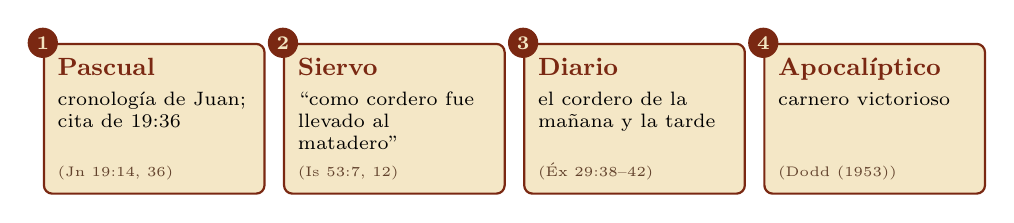
\begin{tikzpicture}
 \foreach \x/\n/\t/\d/\r in {0/1/{Pascual}/{cronología de Juan; cita de 19:36}/{Jn 19:14, 36}, 3.05/2/{Siervo}/{``como cordero fue llevado al matadero''}/{Is 53:7, 12}, 6.1/3/{Diario}/{el cordero de la mañana y la tarde}/{Éx 29:38--42}, 9.15/4/{Apocalíptico}/{carnero victorioso}/{Dodd (1953)}}{
  \node[caja,anchor=north] (b\n) at (\x,0) {\parbox[t][1.55cm][t]{2.45cm}{\RaggedRight
    {\small\textbf{\textcolor{tierraroja}{\t}}}\\[3pt]\scriptsize \d\par\vfill{\tiny\color{sepia}(\r)}}};
  \node[circle,fill=tierraroja,text=papiro,font=\scriptsize\bfseries,inner sep=1.6pt] at (b\n.north west) {\n};}
\end{tikzpicture}\par\medskip
\small\RaggedRight Las dos primeras tienen más apoyo en el evangelio y \destacar{no se excluyen} (Keener, 2003). La serie lee en clave pascual. Juan estructura el ministerio con tres Pascuas (2:13; 6:4; 11:55).
\end{frame}

\begin{frame}{``Esta pascua antes que padezca''}
\begin{columns}[c,onlytextwidth]
\begin{column}{0.53\textwidth}
\begin{cita}¡Cuánto he deseado comer con vosotros esta pascua antes que padezca! Porque os digo que no la comeré más, hasta que se cumpla en el reino de Dios.\fuente{(Lc 22:15--16)}\end{cita}
\begin{cita}Esto es mi cuerpo, que por vosotros es dado; haced esto en memoria de mí.\fuente{(Lc 22:19)}\end{cita}
\end{column}
\begin{column}{0.45\textwidth}\small
\begin{itemize}
\item \destacar{Memoria}: \grc{ἀνάμνησις} = \emph{zikarón} (Éx 12:14).
\item \destacar{Sangre del pacto}: Éx 24:8; Jer 31:31; Mt 26:28.
\item \destacar{Himno}: ``cuando hubieron cantado el himno'' (Mt 26:30), probablemente el \emph{Hallel}.
\item Jesús no interpreta el cordero, sino \destacar{el pan y la copa}.
\end{itemize}
\end{column}
\end{columns}
\end{frame}

\begin{frame}{Éxodo 12 y la Pasión}
\scriptsize\renewcommand{\arraystretch}{1.12}
\begin{tabular}{@{}L{3.4cm}L{1.5cm}L{4.8cm}L{1.9cm}@{}}
\toprule
\textbf{Éxodo 12} & \textbf{Texto} & \textbf{Pasión de Jesús} & \textbf{Texto} \\ \midrule
Se escoge el cordero el día 10 & Éx 12:3 & Entrada en Jerusalén (lectura tipológica) & Jn 12:1, 12 \\
\emph{Seh tamim}, sin defecto & Éx 12:5 & ``Cordero sin mancha''; ``no hallo en él ningún delito'' & 1~P 1:19; Jn 18:38 \\
Inmolado el 14 por la tarde & Éx 12:6 & Muere en la ``preparación de la pascua'' & Jn 19:14 \\
Sangre con hisopo & Éx 12:22 & Esponja ``en un hisopo'' & Jn 19:29 \\
``Ni quebraréis hueso suyo'' & Éx 12:46 & ``No será quebrado hueso suyo'' & Jn 19:36 \\
``Os será en memoria'' & Éx 12:14 & ``Haced esto en memoria de mí'' & Lc 22:19 \\
Salida de la servidumbre & Éx 12:41 & ``Rescatados\ldots{} con la sangre preciosa'' & 1~P 1:18--19 \\
\bottomrule
\end{tabular}\par\smallskip
\precision{las filas 1 y 3 dependen de la cronología joánica y de una lectura tipológica (Chumney, 1994; Baker, 2013); las demás se apoyan en citas o alusiones explícitas.}
\end{frame}

\begin{frame}{Pablo y Pedro}
\begin{columns}[t,onlytextwidth]
\begin{column}{0.50\textwidth}
\begin{cita}Así que celebremos la fiesta, no con la vieja levadura, ni con la levadura de malicia y de maldad, sino con panes sin levadura, de sinceridad y de verdad.\fuente{(1~Co 5:8)}\end{cita}
\scriptsize\RaggedRight Orden pascual: primero el cordero (\grc{ἐτύθη}, hecho cumplido), después la vida sin levadura (\grc{ἑορτάζωμεν}). En 1~Co 10:10 reaparece ``el destructor'' (Fee, 1987).
\end{column}
\begin{column}{0.48\textwidth}
\begin{cita}Fuisteis rescatados\ldots{} no con cosas corruptibles, como oro o plata, sino con la sangre preciosa de Cristo, como de un cordero sin mancha y sin contaminación.\fuente{(1~P 1:18--19)}\end{cita}
\scriptsize\RaggedRight \grc{ἐλυτρώθητε}: el verbo del éxodo (Éx 6:6) y del rescate de los primogénitos (13:13); \grc{ἄμωμος} = \emph{tamim}. He 11:28: Moisés celebró la Pascua ``por la fe''.
\end{column}
\end{columns}
\end{frame}

\begin{frame}{El Cordero como inmolado}
\begin{columns}[c,onlytextwidth]
\begin{column}{0.55\textwidth}
\begin{cita}Y miré, y vi que en medio del trono y de los cuatro seres vivientes, y en medio de los ancianos, estaba en pie un Cordero como inmolado\ldots\fuente{(Ap 5:6)}\end{cita}
\begin{cita}\ldots{}porque tú fuiste inmolado, y con tu sangre nos has redimido para Dios, de todo linaje y lengua y pueblo y nación.\fuente{(Ap 5:9)}\end{cita}
\end{column}
\begin{column}{0.43\textwidth}\small\RaggedRight
\begin{itemize}\small
\item ``En pie'' y ``como inmolado'' (\grc{ὡς ἐσφαγμένον}): \destacar{víctima y vencedor}.
\item Del trono (Ap 4) al Cordero (Ap 5): la adoración se extiende a él (5:12).
\item Nuevo éxodo: plagas, ``cántico de Moisés\ldots{} y del Cordero'' (15:3) (Bauckham, 1993).
\end{itemize}
\precision{Apocalipsis no nombra la Pascua; la tipología se apoya en el Cordero inmolado, la sangre que redime y los ecos del éxodo.}
\end{column}
\end{columns}
\end{frame}

% ==================================================================
\section{Tradición}

\begin{frame}{El \emph{séder} rabínico}
\begin{columns}[t,onlytextwidth]
\begin{column}{0.54\textwidth}\small
\begin{itemize}
\item \textbf{Cuatro copas} (m.~Pesajim 10:1), ligadas a los cuatro verbos de Éx 6:6--7 (Talmud de Jerusalén).
\item \textbf{\emph{Ma nishtaná}}: ``¿Por qué esta noche es distinta?'' (10:4); se explica Dt 26:5--8.
\item \textbf{Rabán Gamaliel}: hay que decir \emph{pésaj}, \emph{matsá} y \emph{maror}; ``en cada generación\ldots{} como si él hubiera salido de Egipto'' (10:5).
\item \textbf{Cuatro noches} del Targum a Éx 12:42 (Le Déaut, 1963).
\end{itemize}
\end{column}
\begin{column}{0.44\textwidth}
\begin{tcolorbox}[colback=mostaza!10,colframe=mostaza!85!tierraroja,boxrule=0.6pt,arc=2pt,title={Precisión: lo tardío},fonttitle=\bfseries\scriptsize,coltitle=caferojizo,colbacktitle=mostaza!30,fontupper=\scriptsize]
Son medievales o modernas las tres \emph{matsot} y el \emph{afikomán} escondido (en la Misná, \emph{afikomán} es la sobremesa que no se añade, 10:8), la copa de Elías y ``el año próximo en Jerusalén''. Las lecturas cristianas de la \emph{matsá} ``rayada y perforada'' (Baker, 2013) son devocionales, no exégesis del texto bíblico.
\end{tcolorbox}
\end{column}
\end{columns}
\end{frame}

% ==================================================================
\section{Debates}

\begin{frame}{Pascua y Cena del Señor}
\scriptsize\renewcommand{\arraystretch}{1.12}
\begin{tabular}{@{}L{3.0cm}L{6.2cm}L{2.9cm}@{}}
\toprule
\textbf{Postura} & \textbf{Tesis} & \textbf{Representantes} \\ \midrule
Memorial anual & Pascua del Nuevo Pacto, 14 de Nisán; pan, vino, lavamiento de pies & Serie; IDDU (2011); cuartodecimanos \\
Memorial & Recuerda y proclama la muerte; los elementos son signos & Zuinglio; bautistas \\
Presencia espiritual & Cristo se da por el Espíritu en la Cena & Calvino; reformados \\
Presencia real y sacrificio & Hace presente el único sacrificio de Cristo & Trento; católicos \\
Cumplimiento escatológico & La memoria pide la venida del reino (``hasta que él venga'') & Jeremias (1966) \\
\bottomrule
\end{tabular}\par\medskip
\small\RaggedRight La \grc{ἀνάμνησις} bíblica \destacar{actualiza} y \destacar{mira hacia adelante} (Lc 22:16; 1~Co 11:26). En esto coinciden la serie y Jeremias; difieren en la frecuencia y la forma.
\end{frame}

\begin{frame}{¿Un sacrificio expiatorio?}
\begin{columns}[t,onlytextwidth]
\begin{column}{0.49\textwidth}\scriptsize\RaggedRight
\textbf{\small\textcolor{tierraroja}{No expiatorio en Éx 12}}
\begin{itemize}\scriptsize
\item \heb{זֶבַח} (\emph{zevaj}, se come), no \heb{חַטָּאת} (\emph{jatat}).
\item La familia come toda la carne.
\item Sangre en la puerta, no en un altar: señal protectora.
\item No se habla de pecado (Propp, 1999; Sarna, 1991).
\end{itemize}
\end{column}
\begin{column}{0.49\textwidth}\scriptsize\RaggedRight
\textbf{\small\textcolor{tierraroja}{Sustitutivo y expiatorio}}
\begin{itemize}\scriptsize
\item Donde hay sangre no muere el hijo: \destacar{muerte en lugar de otro}.
\item Lv 17:11; sangre al altar en el templo (2~Cr 35:11); \emph{jatat} el 14 (Ez 45:22).
\item NT: ``quita el pecado'' (Jn 1:29); ``para remisión de los pecados'' (Mt 26:28).
\end{itemize}
\end{column}
\end{columns}
\medskip
\begin{tcolorbox}[colback=papiro,colframe=tierraroja,boxrule=0.8pt,arc=2pt,fontupper=\scriptsize]
\textbf{Síntesis posible.} En Éxodo 12 la Pascua es un sacrificio de comunión cuya sangre protege por sustitución. En el NT, Cristo cumple a la vez la Pascua, el pacto (Éx 24:8) y la expiación (Is 53; Lv 16), sin confundir las figuras (Dunn, 1998; Wright, 2013).
\end{tcolorbox}
\end{frame}

% ==================================================================
\section{Síntesis}

\begin{frame}{Pésaj: definición y aportes}
\begin{tcolorbox}[colback=papiro,colframe=tierraroja,boxrule=1pt,arc=3pt,fontupper=\scriptsize]
La Pascua es la solemnidad del 14 de Abib, ``entre las dos tardes'' (Lv 23:5), \destacar{memorial perpetuo} (Éx 12:14) de la noche en que el \SENOR{} juzgó a Egipto, \destacar{vio la sangre} y \destacar{pasó por encima} de las casas de Israel (Éx 12:13, 27). El Nuevo Testamento la ve cumplida en Jesús, ``nuestra pascua'' (1~Co 5:7), cuyo memorial se celebra ``hasta que él venga'' (1~Co 11:26).
\end{tcolorbox}
\scriptsize\renewcommand{\arraystretch}{1.08}
\begin{tabular}{@{}L{2.0cm}L{10.1cm}@{}}
\toprule
\textbf{Lectura} & \textbf{Aporte} \\ \midrule
Histórica & Mes de las espigas y luna llena; juicio sobre Egipto; Pascua en cada refundación de Israel. \\
Filológica & \emph{Pésaj} = saltar y proteger; \emph{ot}, señal ``para vosotros''; \emph{maror} y \emph{avodá}; \grc{πάσχα}. \\
Textual & 430 años (TM/LXX/PS); Dt 16:7 y 2~Cr 35:13; Jn 19:36; fecha de la cena abierta. \\
Literaria & Ley y relato entrelazados; preguntas de los hijos; nuevo éxodo (Is 52:12). \\
La serie & Memorial de los primogénitos; el rito es la víctima; la Cena ``hasta que él venga''. \\
\bottomrule
\end{tabular}
\end{frame}

% ==================================================================
\section{Reflexión}

\begin{frame}{Para la reflexión}
\small
\begin{enumerate}
\item La familia debía quedarse \destacar{dentro} ``hasta la mañana'' (Éx 12:22). ¿Qué significa permanecer en la casa marcada por la sangre de Cristo, y no solo haberla marcado una vez?
\item La sangre fue señal ``para vosotros'' (12:13). ¿Descansa usted en lo que Dios ve, o en lo que siente? (He 11:28).
\item ``Lo contarás en aquel día a tu hijo'' (13:8). ¿Cómo responde, \destacar{con su historia}, a quien pregunta ``¿qué rito es este?''
\item Los librados de la muerte pertenecen a Dios (13:2; 1~Co 6:19--20). ¿Qué trata todavía como propio?
\item Antes del memorial, ¿qué ``levadura de malicia y de maldad'' debe quitar (1~Co 5:8)?
\end{enumerate}
\end{frame}

% ==================================================================
\section{Glosario}

\begin{frame}{Glosario}
\scriptsize
\begin{columns}[t,onlytextwidth]
\begin{column}{0.49\textwidth}
\begin{description}\setlength{\itemsep}{1pt}
\item[Abib] (\heb{אָבִיב}) espiga verde; primer mes.
\item[\emph{Avodá}] (\heb{עֲבֹדָה}) servidumbre; ``rito''.
\item[\emph{Bein ha'arbayim}] (\heb{בֵּין הָעַרְבָּיִם}) entre las dos tardes.
\item[\emph{Leil shimurim}] (\heb{לֵיל שִׁמֻּרִים}) noche de guardar.
\item[\emph{Maror}] (\heb{מָרוֹר}) hierba amarga.
\item[\emph{Mashjit}] (\heb{מַשְׁחִית}) destructor.
\end{description}
\end{column}
\begin{column}{0.49\textwidth}
\begin{description}\setlength{\itemsep}{1pt}
\item[\emph{Ot}] (\heb{אוֹת}) señal.
\item[\emph{Pascha}] (\grc{πάσχα}) transcripción griega.
\item[\emph{Pésaj}] (\heb{פֶּסַח}) Pascua; ``pasar, proteger''.
\item[\emph{Seh tamim}] (\heb{שֶׂה תָמִים}) res menor sin defecto.
\item[\emph{Zevaj}] (\heb{זֶבַח}) sacrificio que se come.
\item[\emph{Zikarón}] (\heb{זִכָּרוֹן}) memoria; \grc{ἀνάμνησις}.
\end{description}
\end{column}
\end{columns}
\end{frame}

% ==================================================================
\section{Referencias}

\begin{frame}{Referencias}
\fontsize{5.6}{6.6}\selectfont
\begin{columns}[t,onlytextwidth]
\begin{column}{0.49\textwidth}
\refapa{Baker, D. (2013). \emph{El poder espiritual de las siete fiestas de Dios}. Editorial Imagen.}
\refapa{Bauckham, R. (1993). \emph{The climax of prophecy}. T\&T Clark.}
\refapa{Bokser, B.~M. (1984). \emph{The origins of the Seder}. University of California Press.}
\refapa{Brown, R.~E. (1994). \emph{The death of the Messiah} (2 vols.). Doubleday.}
\refapa{Chumney, E. (1994). \emph{The seven festivals of the Messiah}. Destiny Image.}
\refapa{Dodd, C.~H. (1953). \emph{The interpretation of the Fourth Gospel}. Cambridge University Press.}
\refapa{Dunn, J.~D.~G. (1998). \emph{The theology of Paul the apostle}. Eerdmans.}
\refapa{Elliger, K., \& Rudolph, W. (Eds.). (1997). \emph{Biblia Hebraica Stuttgartensia} (5.ª ed.). Deutsche Bibelgesellschaft.}
\refapa{Eusebio de Cesarea. (1973). \emph{Historia eclesiástica} (A. Velasco-Delgado, Trad.). BAC.}
\refapa{Fee, G.~D. (1987). \emph{The first epistle to the Corinthians} (NICNT). Eerdmans.}
\refapa{Hoffmeier, J.~K. (1997). \emph{Israel in Egypt}. Oxford University Press.}
\refapa{Humphreys, C.~J. (2011). \emph{The mystery of the Last Supper}. Cambridge University Press.}
\refapa{Iglesia de Dios Unida. (2011). \emph{Las fiestas santas de Dios}. Autor.}
\refapa{Jaubert, A. (1957). \emph{La date de la Cène}. Gabalda.}
\refapa{Jeremias, J. (1966). \emph{The eucharistic words of Jesus}. SCM Press.}
\end{column}
\begin{column}{0.49\textwidth}
\refapa{Josefo, F. (1997). \emph{Antigüedades judías} (J. Vara Donado, Trad.). Akal.}
\refapa{Josefo, F. (1999). \emph{La guerra de los judíos: Libros IV--VII} (J.~M. Nieto Ibáñez, Trad.). Gredos.}
\refapa{Keener, C.~S. (2003). \emph{The Gospel of John} (2 vols.). Hendrickson.}
\refapa{Le Déaut, R. (1963). \emph{La nuit pascale}. Institut Biblique Pontifical.}
\refapa{Meier, J.~P. (1991). \emph{A marginal Jew} (Vol. 1). Doubleday.}
\refapa{Nestle, E., \& Aland, K. (Eds.). (2012). \emph{Novum Testamentum Graece} (28.ª ed.). Deutsche Bibelgesellschaft.}
\refapa{Porten, B., \& Yardeni, A. (1986). \emph{Textbook of Aramaic documents from ancient Egypt} (Vol. 1). Hebrew University.}
\refapa{Propp, W.~H.~C. (1999). \emph{Exodus 1--18} (AB 2). Doubleday.}
\refapa{Rahlfs, A., \& Hanhart, R. (Eds.). (2006). \emph{Septuaginta}. Deutsche Bibelgesellschaft.}
\refapa{Sarna, N.~M. (1991). \emph{Exodus} (JPS Torah Commentary). Jewish Publication Society.}
\refapa{Sociedades Bíblicas en América Latina. (1960). \emph{Santa Biblia: Reina-Valera 1960}.}
\refapa{Tigay, J.~H. (1996). \emph{Deuteronomy} (JPS Torah Commentary). Jewish Publication Society.}
\refapa{VanderKam, J.~C. (1998). \emph{Calendars in the Dead Sea Scrolls}. Routledge.}
\refapa{Wright, N.~T. (2013). \emph{Paul and the faithfulness of God}. Fortress Press.}
\end{column}
\end{columns}
\par\smallskip{\color{sepia}Citas bíblicas: Reina-Valera 1960, con \SENOR{} donde dice ``Jehová''. Hebreo: BHS; griego: NA28 y LXX. Misná, Talmud, Targum y Rashi desde Sefaria y Danby (1933).}
\end{frame}

\end{document}
